\newpage
\section {Интеграция ИНС/ГНСС}

 
 Основной целью интеграции кластерного инерциального блока с навигационным приемником является повышение
 надежности и точности решения. Для обеспечения максимальной надёжности интегрированного алгоритма позиционирования необходимо воспользоваться соответсвующей схемой интеграции двух систем. 
 В данной работе используется OEM плата спутникового навигационного приемника компании NTLab. Данная плата позволяет пользователю получить доступ к срезу кодовых и фазовых измерений на текущую эпоху. Таким образом, тесная схема интеграции ИНС и СНС, которая предполагает использование псевдодальностей СНС и псевдодальности ИНС, видится наиболее оптимальным вариантом. 
 
 
 На рисунке (Рис. 10) представлена схема тесной интеграции БИНС на базе кластерного чувствительного элемента и спутникового навигационного приемника. 

 \begin{figure}[h!]
 	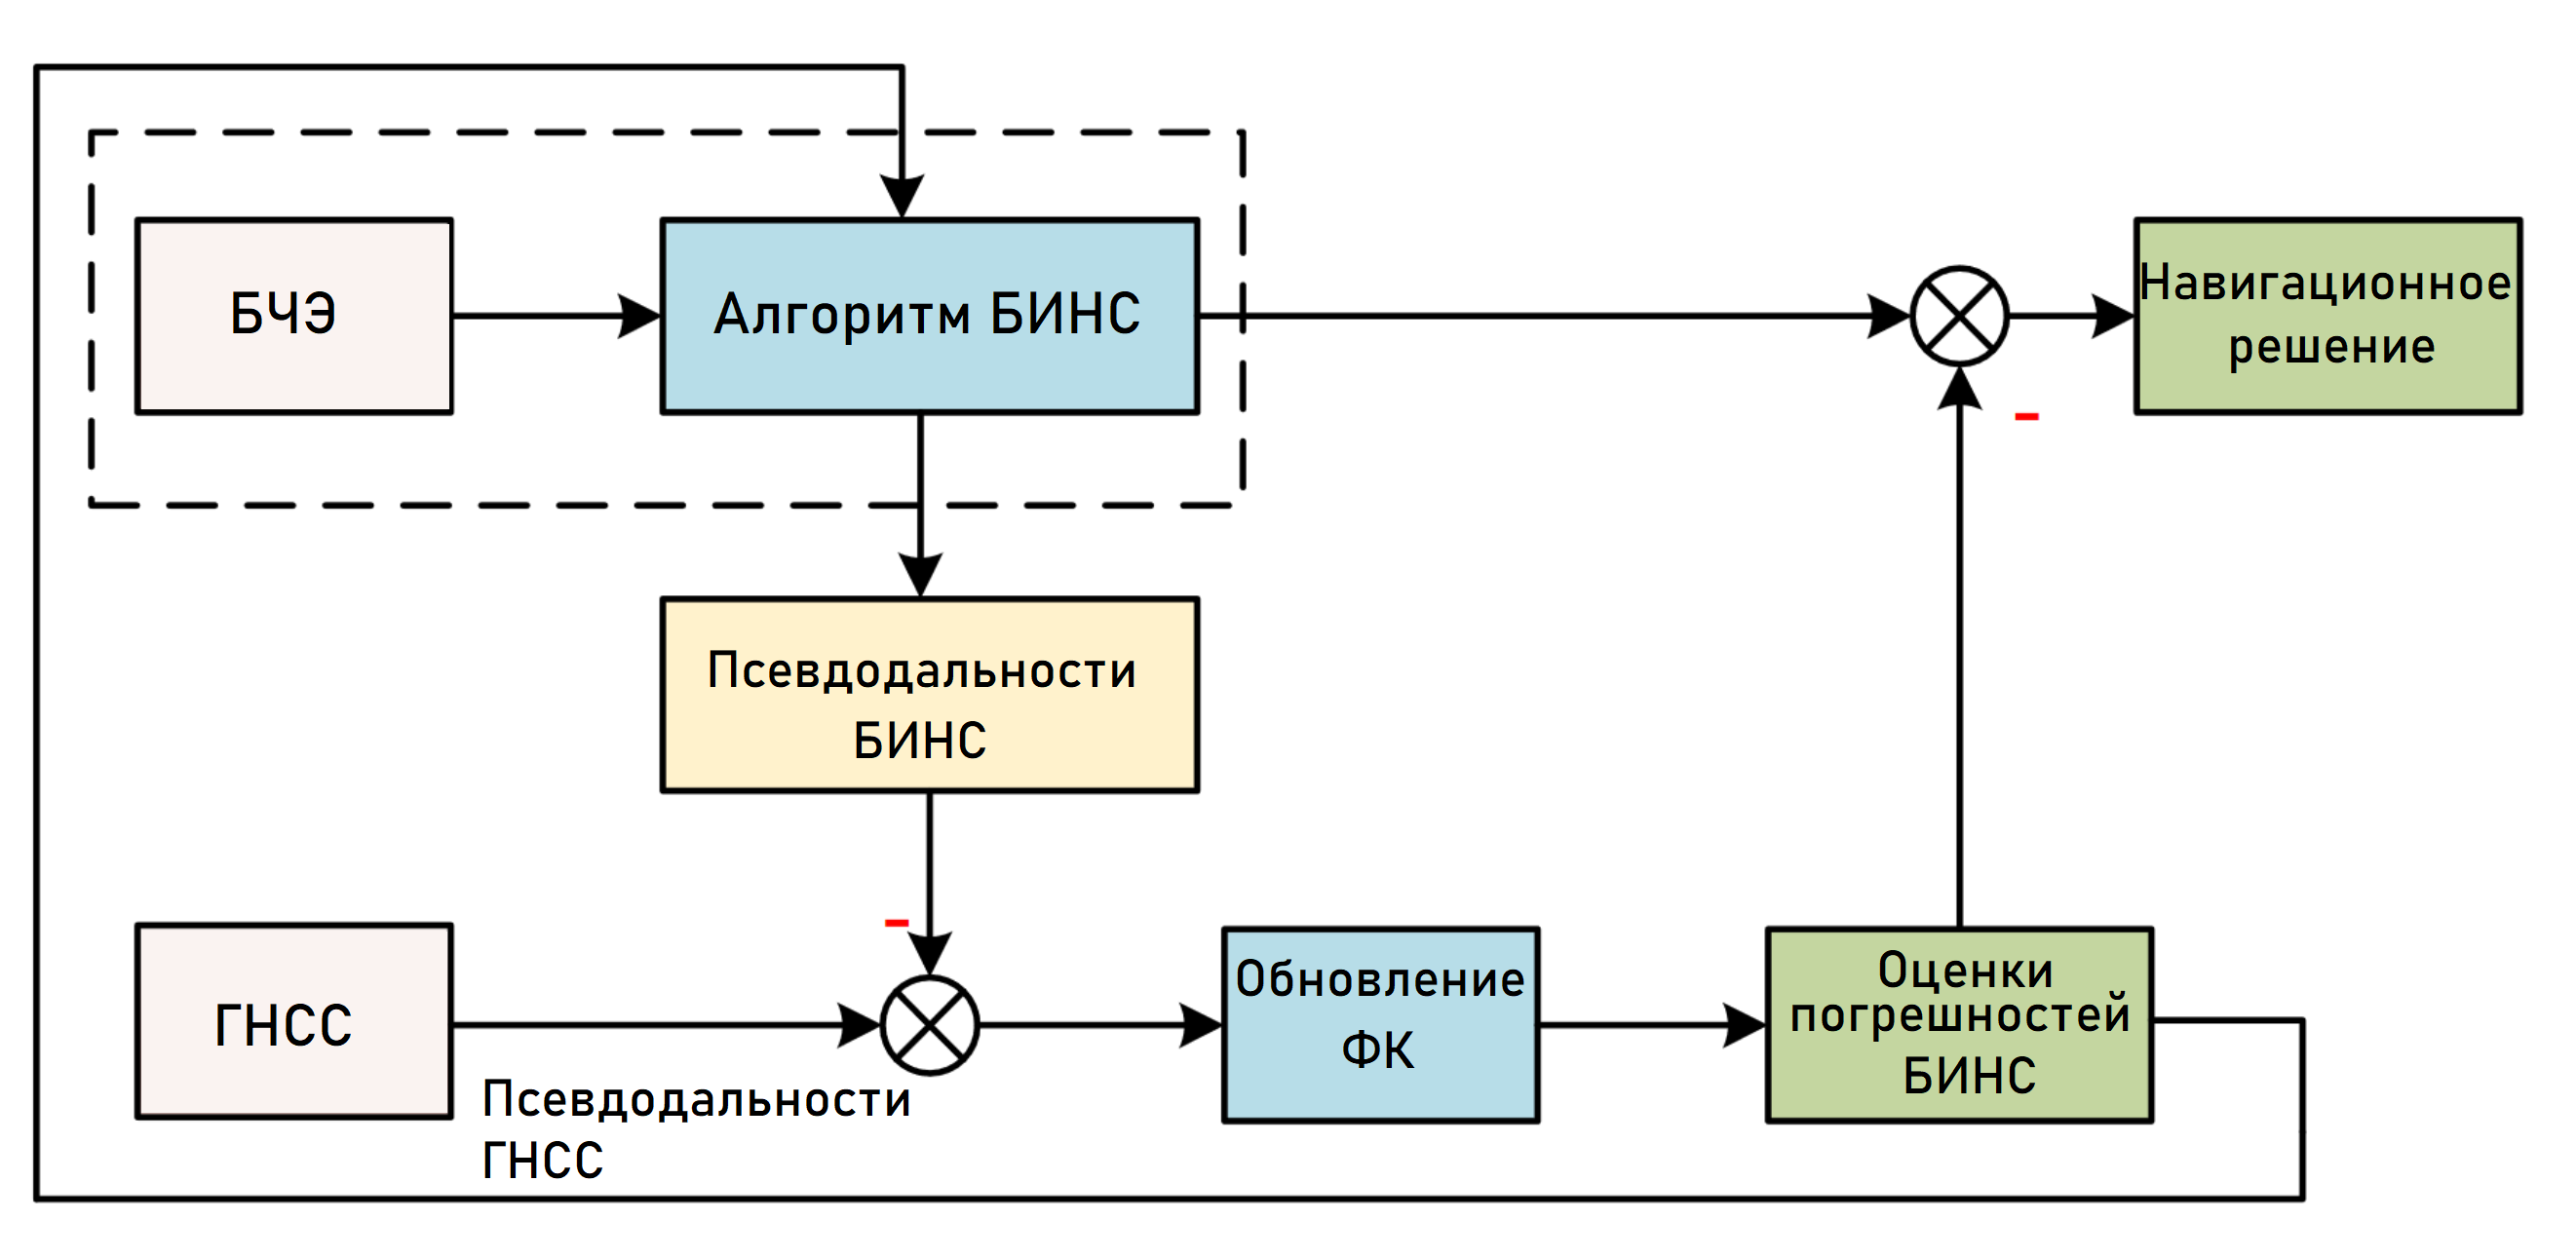
\includegraphics[width=1.0\linewidth]{integration.png}
 	\label{fig:integration}
 	\caption{\label{fig:cluster_pcb} Схема интеграции ИНС/ГНСС}
 \end{figure}


Алгоритм БИНС представлен системой уравнений: 


	\begin{equation} \label{eq:tr_mat}
		\begin{gathered}
			\begin{split}
				& \bm C_b^e(+) = \bm C_b^e(-) \bm C_{b+}^{b-} - \bm \Omega_e \bm C_b^e(-) \tau_{ins} \\
				&  \bm C_{b+}^{b-} = I_3 + \sin \alpha (\alpha \times) / \alpha + (1 - \cos \alpha )(\bm \alpha \times)^2 / \alpha^2 \\ 
				& \bm \alpha =  \bm \omega\tau_{ins}, \alpha = \parallel \bm \alpha \parallel
			\end{split}
		\end{gathered}
	\end{equation}
	
	\begin{equation}
		\label{eq:vel}
		\begin{split}
			& \bm v_{ins} (+) = \bm v_{ins}(-) + (\bm f_e + \bm g (\bm r_{ins}(-) - 2 \bm \Omega_e \bm v_{ins} (-) ) )  \tau_{ins} \\
			& \bm f_{ins} = (\bm C_b^e(-) \bm C_b^e(+)) \bm f / 2
		\end{split}
	\end{equation}	
	
	\begin{equation}
		\label{eq:coord}
		\bm r_{ins}(+) = \bm r_{ins}(-) + (\bm v_{ins}(-) + \bm v_{ins}(+)) \tau_{ins}/2
	\end{equation}


Вектор состояния, подлежаший оцениванию: 
	
\begin{equation} 
	\label{eq:state_vector}
	x = (\delta \psi_{ins} ^ T, \delta r_{ins} ^ T, \delta v_{ins} ^ T, 
	b_{a} ^ T, b_{g} ^ T) ^ T
\end{equation} 

\vspace{0.5cm}

где:  \\ 
	
	{ \large $ \delta \psi_{ins} $ } - ошибка определения ориентации;


    { \large $ \delta r_{ins} $ }    - ошибка определения координат; 
    
    
    { \large $ \delta v_{ins} $ }    - ошибка определения скорости;  
    
    
    { \large $ \delta v_{ins} $ }    - смещение нуля акселерометров; 
   
    
    { \large $ b_{g} $ }             - дрейф гироскопов; \\
    

Для схемы тесной интеграции модель измерений представлена следующим образом: 

\begin{equation}
	\label{eq:ins_19}
	h(\hat{x}) = (h_p(\hat{x})^T, h_{\dot{p}}(\hat{x})^T)^T
\end{equation}

\begin{equation*}
	h_p(\hat{x}) = 
	\begin{pmatrix}
		\rho_r^{12} - cdT^{12} \\
		\rho_r^{13} - cdT^{13} \\
		\vdots \\ 
		\rho_r^{1m} - cdT^{1m} \\
	\end{pmatrix}
	,
	h_{\dot{p}}(\hat{x}) = 
	\begin{pmatrix}
		\dot{\rho}_r^{12} - cd\dot{T}^{12} \\
		\dot{\rho}_r^{13} - cd\dot{T}^{13} \\
		\vdots \\ 
		\dot{\rho}_r^{1m} - cd\dot{T}^{1m} \\
	\end{pmatrix}
\end{equation*}

\begin{equation}
	\label{eq:ins_20}
	H(\hat{x}) = \frac{\partial h(x)}{\partial x}\bigg{|}_{x=\hat{x}} = 
	\begin{pmatrix}
		0 & -DE & 0 & 0 & 0 \\ 
		0 & 0 & -DE & 0 & 0
	\end{pmatrix}
\end{equation}

Матрица обновления состояния системы: 

	\begin{equation}
		\label{eq:ins_21}
		F_k^{k+1} = 
		\begin{pmatrix}
			I_3 - \Omega_e \tau_r & 0 & 0 & 0 & \hat{C}_b^e \tau_r\\
			0 & I_3 & I_3 \tau_r & 0 & 0 \\
			-(\hat{C}_b^e f \times) \tau_r & 0 & I_3 - \Omega_e \tau_r & \hat{C}_b^e \tau_r & 0\\
			0 & 0 & 0 & I_3 & 0 \\
			0 & 0 & 0 & 0 & I_3 \\
		\end{pmatrix}
	\end{equation}

Разрешая данные уравнения на каждом такте работы фильтра Калмана, мы получим оценку вектора состояния из уравнения \ref{eq:state_vector}. Оценка даннного вектора затем будет использована в качестве модели динамики объекта, чьи координаты подлежат оцениванию в фильтре RTK. 


Рассмотрим этап прогноза фильтра Калмана для оценки приращений позиции в режиме RTK:  

\begin{equation}
	\label{eq:rk_gnss}
	\begin{split}
		& { \hat{r}_{r,k+1}(-) = \hat{r}_{r,k}(+) + (\hat{\nu}_{ins/gps,k+1} + \hat{\nu}_{ins/gps,k})\tau_r/2 } \\
		& { \hat{\nu}_{r,k+1}(-) = \hat{\nu}_{ins/gps,k+1} }\\
		& {P}_{k+1} = {F}_k^{k+1} {P}_k(+) {F}_k^{k+1^T} + {Q}_k^{k+1}
	\end{split}
\end{equation}

\begin{equation*}
	\label{eq:Fk_gnss}
	{F}_k^{k+1} = 
	\begin{pmatrix}
		{I}_3 & & & \\
		& 0 & & \\
		& & {I}_{m-1} & \\
		& & & {I}_{m-1}
	\end{pmatrix}
\end{equation*}

\begin{equation*}
	\label{eq:Q_k}
	{Q}_k^{k+1} = 
	\begin{pmatrix}
		{P}_{\nu-ins/gps,k+1} \tau_r & & & \\
		& {P}_{\nu-ins/gps,k+1}  & & \\
		& & 0 & \\
		& & & 0
	\end{pmatrix}
\end{equation*}	

Как видно из уравнения \ref{eq:rk_gnss} для априорной оценки приращения координат используются оценки скорости, полученные из алгоритма тесной интеграции СНС и БИНС. Это позволяет создать более детерминированную модель движения объекта и, как следствие, повысить точность оценивания фильтра. 


Таким образом, анализируя невязки, расчитанные с учётом реальной динамики объекта, оцененной при помощи БИНС: 

\begin{equation}
	\label{eq:ins_23.1}
	\nu = y_k - h(\hat{x}_k(-))			
\end{equation}

и воспользовавшись критерием: 

\begin{equation}
	\label{eq:ins_24}
	\nu_i^2 > nq_{i, \nu}
\end{equation}

мы ожидаем повысить процент детектирования скачков в фазовых измерениях. 

\newpage 
 